\documentclass[10pt,a4paper,twocolumn,notitlepage]{article}
\usepackage[latin1]{inputenc}
\usepackage{amsmath}
\usepackage{amsfonts}
\usepackage{amssymb}
\usepackage{titling}
\usepackage{graphicx}
\usepackage[left=2cm,right=2cm,top=2cm,bottom=2cm]{geometry}
\usepackage{hyperref}


\title{Quantitative Assessment Of A Mahlkonig EK-43 Burr Alignment}

\begin{document}
\thispagestyle{empty}

\twocolumn[
  \begin{@twocolumnfalse}
    \maketitle
    
\textbf{Disclosure:}\\
\textit{This project would not be possible without the incredible program written by astrophysicist and specialty coffee brewing enthusiast, J. Gagne, at \url{https://coffeeadastra.com}. Much of his original source code, designed to understand the effects of particle size distribution on coffee taste, was used in the following experiment and can be found at: \url{https://github.com/jgagneastro/coffeegrindsize}. Supplementary code adapts data collected by his coffee grind size app, stored in .csv (comma separated values) files, into a readable form for multiple grind settings.}

    \begin{abstract}
      Recent variability in tasting notes during cupping of brewed coffee lead our team at Flight Coffee Co. Roasting Lab in Bedford, New Hampshire to suspect our Mahlkonig EK-43 Coffee Grinder needed an adjustment. This suspicion was verified using an open source program (discussed and linked in Disclosure). Subsequent burr adjustments made to the Mahlkonig EK-43 significantly improved the grinder's performance and our team's ability to achieve expected and consistent flavor profiles. A secondary portion of this study involved measurement of grind size at each EK-43 grind setting in an effort to compare these settings with settings of different grinders. The would help our team better support customers with different grinders who would like to improve extraction levels and flavor of their coffee. However, the EK-43's current configuration complicated this effort and new burrs will likely be needed to achieve precision in cross-product grind-size comparison. \\\\
    \end{abstract}
  \end{@twocolumnfalse}
]

\section{Introduction}
Over time a primary problem grinders face is burrs dulling and or becoming misaligned as several thousands of pounds of coffee pass through them in commercial settings. Grinders ideally produce a mass of single-size particles at some grind setting. Different grinder designs can aid or hinder this goal. All burr designs will produce a range of particle sizes, some larger and some smaller than the desired size. Quality burr designs and ongoing maintenance aims to minimize variability outside the desired size range. Greater variability can result in poorly or ``variably" extracted coffee, even with all other brew parameters carefully controlled and replicated. Variable-extraction in this context means at the same grind setting the coffee tastes different brew-to-brew. Unfortunately this perception is typically only accounted for anecdotally over time as the grinder ages, and can be influenced by many factors. Typically, data is rarely collected over time to quantify grinder quality changes. Another consequence, or perhaps indication, of an aging grinder is needing to adjust the grind setting finer or coarser to achieve similar brew times.\\

Different coffee particle sizes have different extractable surfaces areas, so a larger variation in size allows larger variation in extraction rate at any point within the coffee slurry. Our Mahlkonig EK-43 grinder, manufactured Aug 2015, exhibited not only a variable flavor profile in brewed coffee but also a seemingly noticeable spread in the grind size to the naked eye. This project aimed to quantify whether our Mahlkonig EK-43 needed realignment and if so how beneficial the alignment was after completion. \\

A program called coffeegrindsize (1) was used to analyze a grind sample and calculate the average diameter and average surface area, as well as the standard deviation to 1$\sigma$. Supplementary Python code (5) was written to expand on the data output from coffeegrindsize which is stored in .csv files to collate many different grind settings. Analyzing the grinder in this way made possible calculating the grinder's setting-change linearity. Ideally this linearity approaches 1 ($R^2=1$) as the only adjustment is the movement of the two burrs with respect to each other. A strong linear fit with minimal variation could allow comparing two grinders by finding, quantitatively, what setting on a test grinder matches the size of our known setting. Additional code is in development to automate grinder-to-grinder correlation in this way. 

Upon initial inspection the burrs were misaligned slightly both axially and radially. The burrs were also notably dull, and should likely be changed sometime soon. Another round of tests will follow if that occurs. After shimming and aligning the faceplate-side burrs using the method described in Barista Hustle's video (4)there was a noticeable improvement in grind pass-through time (less time for residuals to exit the grinding chamber), a seeming improvement in the naked-eye appearance of ground coffee's size uniformity, as well as a qualitative improvement in flavor. Re-taking data post-adjustment shows improvements in both grind quality and grind-setting change linearity. However, given the large spread in grind size distribution, it is unlikely the parameters of the linear fit model can adequately describe particle-size in a grinder-to-grinder comparison to a level more useful than trial-and-error.

\section{Methodology}
11 grind samples of a few grams each were placed into individual cupping bowls. The EK-43 was set to grind setting 1, a purge mass was run through, then the sample was run through and re-collected in the cupping bowl. The coffee was then stirred with a spoon to homogenize the grinds in the cupping bowl. The EK-43 was adjusted to setting two, a purge sample was run through at this new setting, then the sample was run through and re-collected in the cupping bowl. This procedure was repeated for each major grind setting (1-11) with several vigorous knocks on the knock-arm between samples to help purge any coffee grounds from the previous setting. The samples are shown in Figure 1. 
\begin{center}\begin{figure}[h!]
 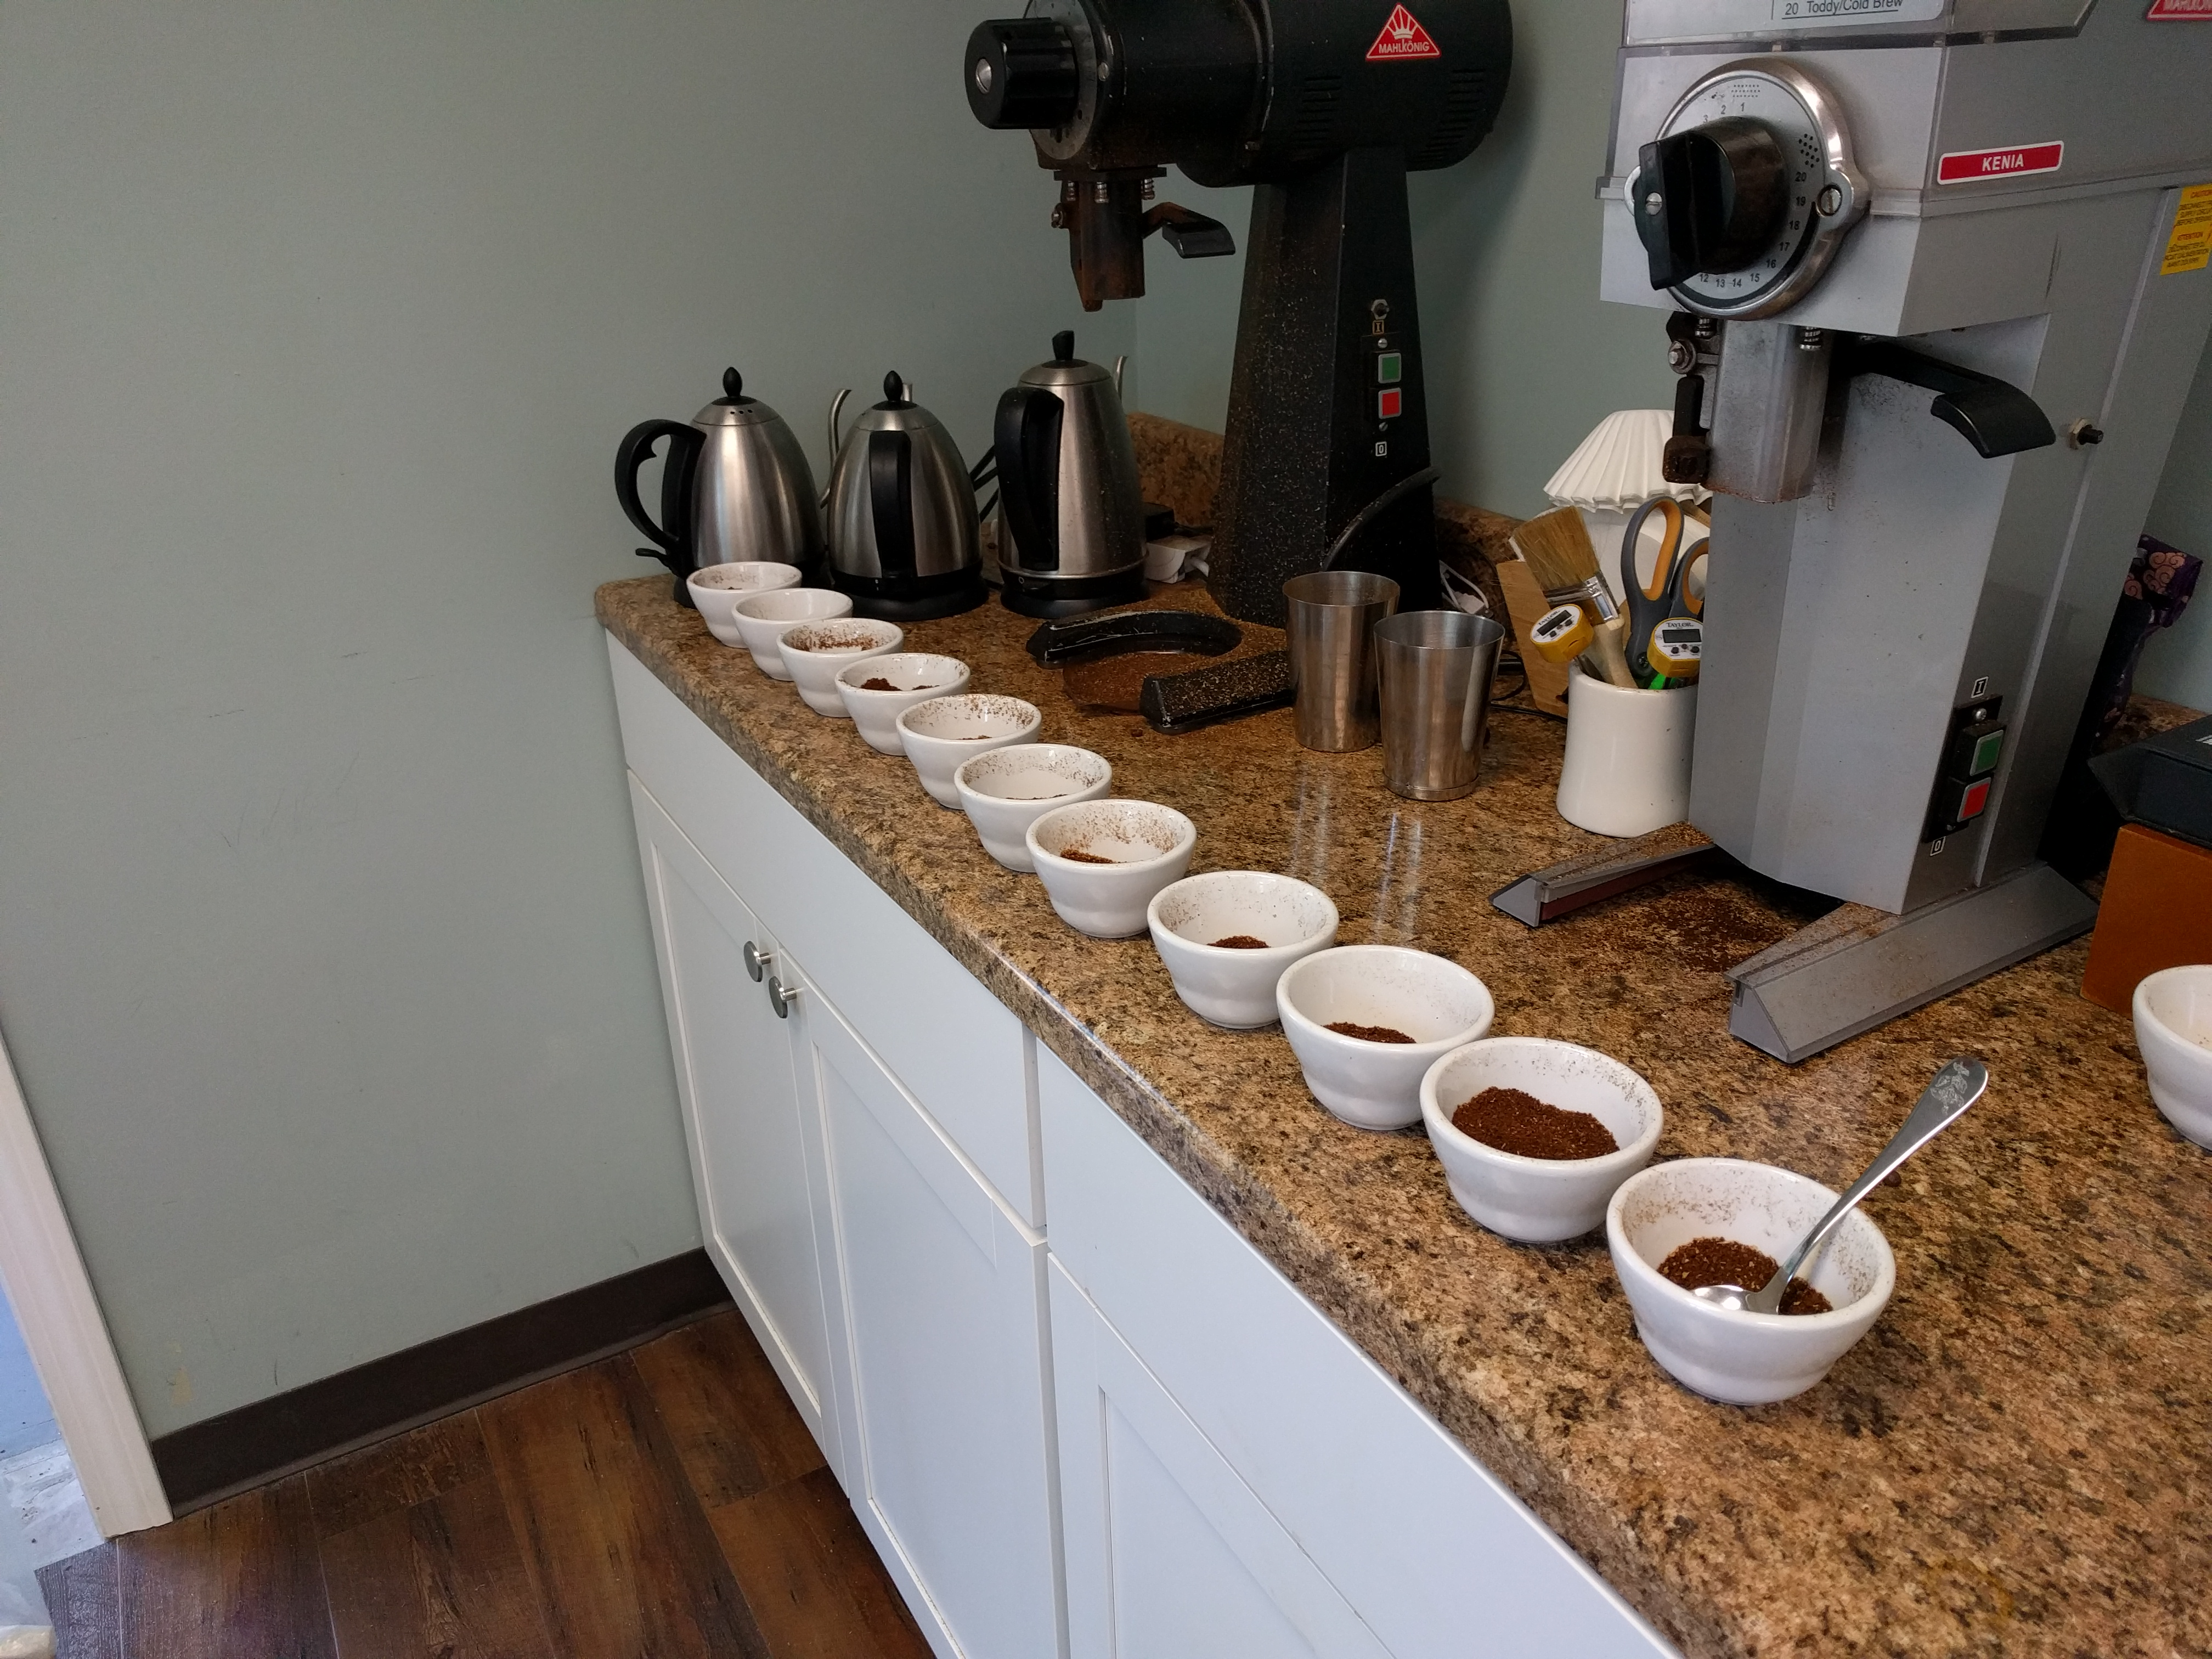
\includegraphics[width=\columnwidth]{preAdjustmentData/IMG_20190831_132715.jpg}
 \caption{Grind samples in cupping bowls}\label{fig:cuppingBowls}\end{figure}\end{center}
A white sheet of paper, labeled with the current grind setting and a reference scale object (a US nickel), was placed on a large white backdrop to provide contrast with the brown coffee grounds. Coffee was spread on the paper as uniformly as possible. Two methods for coffee distribution were tried:

\begin{enumerate}
\item Coffee was shook from a cupping spoon approximately two feet above the surface of the paper to let it fall and bounce.
\item Coffee was pinched from the cupping bowls and sprinkled approximately two feet above the surface of the paper to let it fall and bounce.
\end{enumerate}

Sprinkling the coffee by hand consistently provided more evenly distributed coffee particles on the paper and fewer clumps caused by static, an example image is shown in Figure \ref{fig:grindSample}.

Each image was uploaded into coffeegrindsize and processed following the guide found in J. Gagne's user manual[3] with careful consideration to remove clumps from the data set, shown in Figure \ref{fig:analysisExample}. Pre-adjustment data was processed four times because the coffee was not distributed on the paper as effectively in this first round of testing as compared with post-adjustment. Each setting was fairly consistent between processing attempts even though slightly different analysis regions were used each time. 

\begin{center}\begin{figure}[h!]
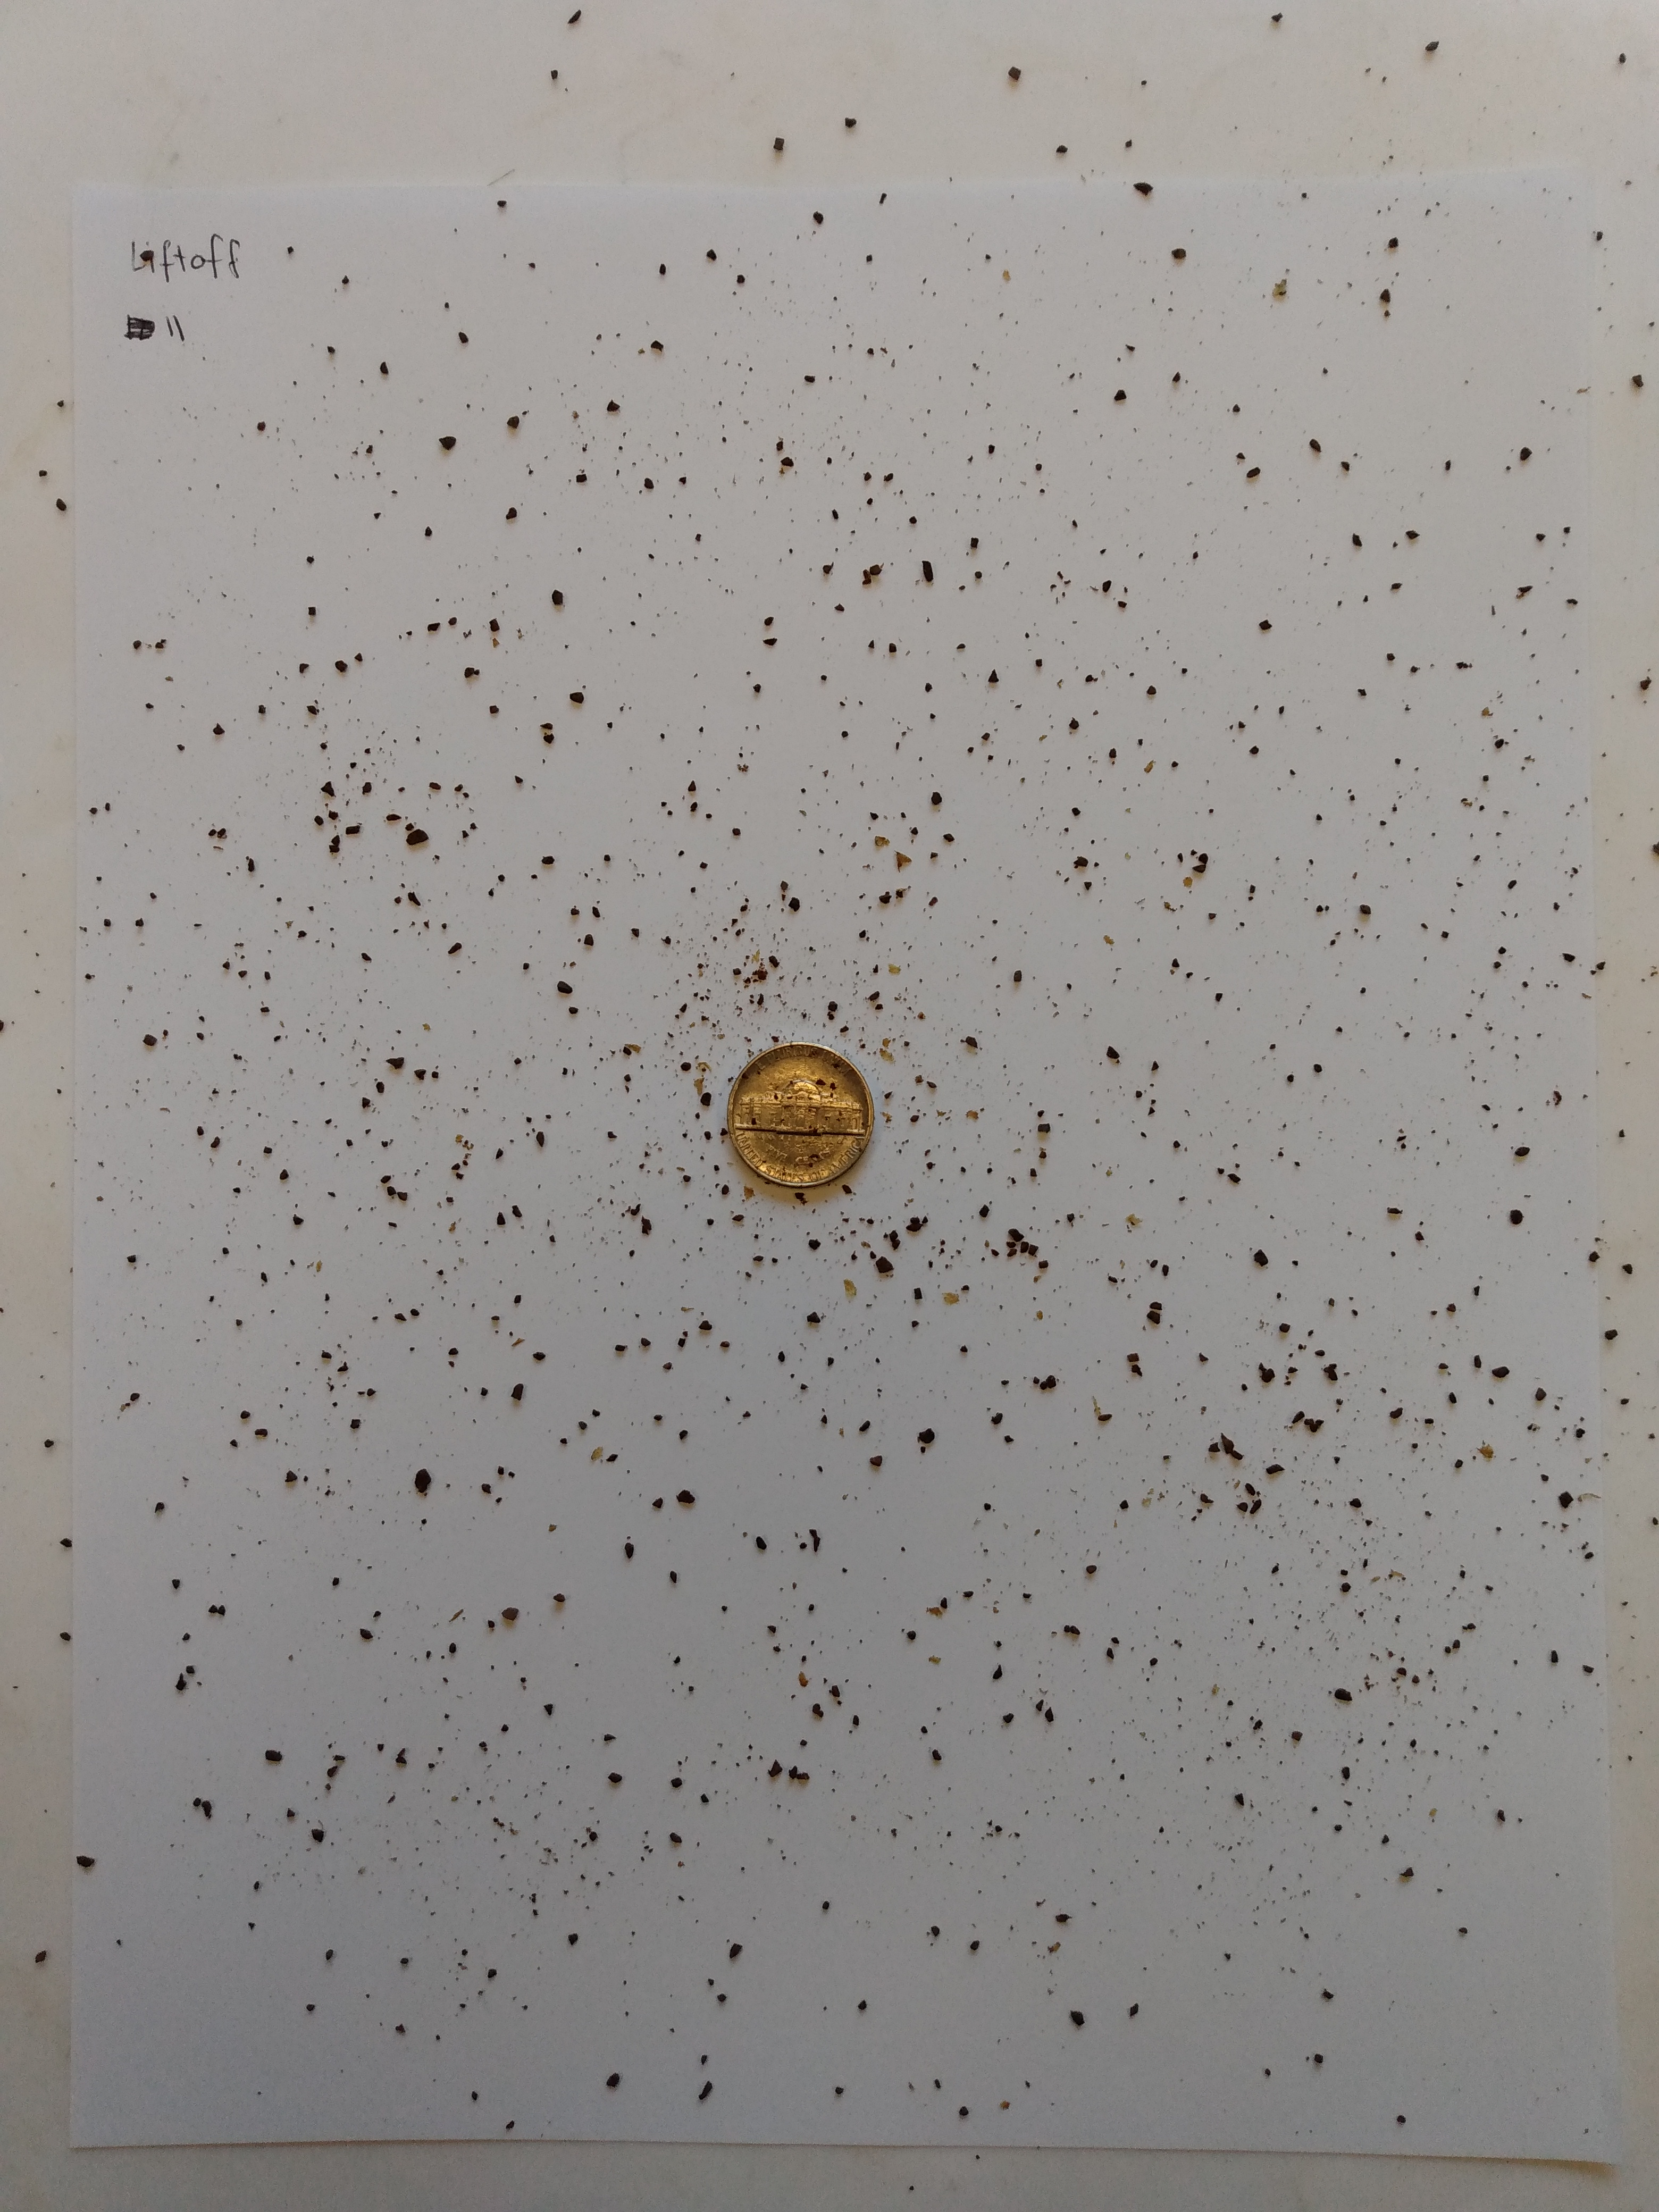
\includegraphics[width=\columnwidth]{postAdjustmentData/IMG_20191005_144811062.jpg}\caption{Coffee spread on paper. This image is analyzed in the coffeegrindsize application.}\label{fig:grindSample}\end{figure}\end{center}
\begin{center}\begin{figure}[h!]
 \includegraphics[width=\columnwidth]{postAdjustmentData/analysisExample.png}
 \caption{Using the coffeegrindsize application}\label{fig:analysisExample}\end{figure}\end{center}

\section{Results}
CSV files generated from coffeegrindsize was passed into the supplementary code and processed. Each grind setting's average diameter and 2D surface area was calculated and stored in arrays as well the 1 $\sigma$ standard deviation from the average. The standard deviation is calculated internally in coffeegrindsize[2] after simulating cumulative density functions left and right of the average value. This section was taken directly from J. Gagne's source code and adapted to work with the supplemental code. The standard deviation values are plotted as error bars above and below the average, as shown in Figure 5. Rather than display skewness and/or kurtosis for each grind setting the higher-value deviation is labeled green to show whether fines or boulder production dominates for a particular grind setting.\\

Once all settings were analyzed the Python module Scipy.curve\_ fit[6] was used to calculate a linear regression through these average values. The parameters follow the general form: $$grindSize = A*grindSetting + B$$ 

\begin{center}
\begin{table}[h]
\resizebox{.83\columnwidth}{!}{ \begin{minipage}{\columnwidth}
\begin{tabular}{|r|c|c|r|}
\hline			
  & Slope (A) & Intercept (B) [mm] & $R^2$ \\ \hline
Pre-Adjustmment & 0.89 +/- .041 & .26 +/- .006 & .96 \\  \hline
Post-Adjustment & 0.068 +/- .022 & .31 +/- 0 .0032 & .98 \\ \hline
\end{tabular}
\end{minipage} }
\end{table}
\end{center}

The average values and linear regression were plotted against grind setting, shown below in Figures \ref{fig:preAdjustmentGraph} and \ref{fig:postAdjustmentGraph}.\\

\begin{center}\begin{figure}[h]
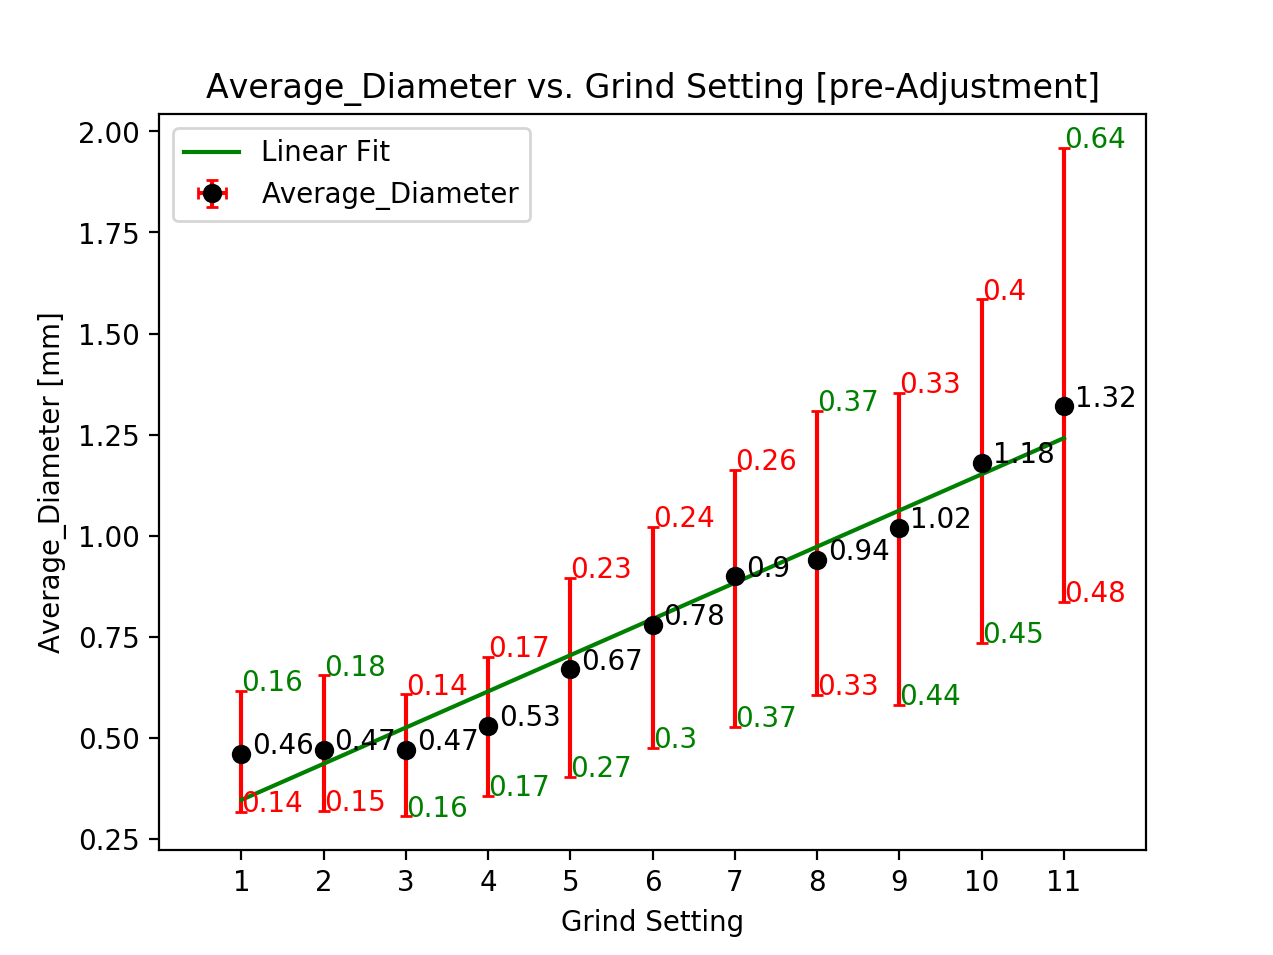
\includegraphics[width=\columnwidth]{preAdjustmentAverage_DiameterPlot.png}\caption{Pre-Adjustment Plot}\label{fig:preAdjustmentGraph}\end{figure}

\begin{figure}[h]
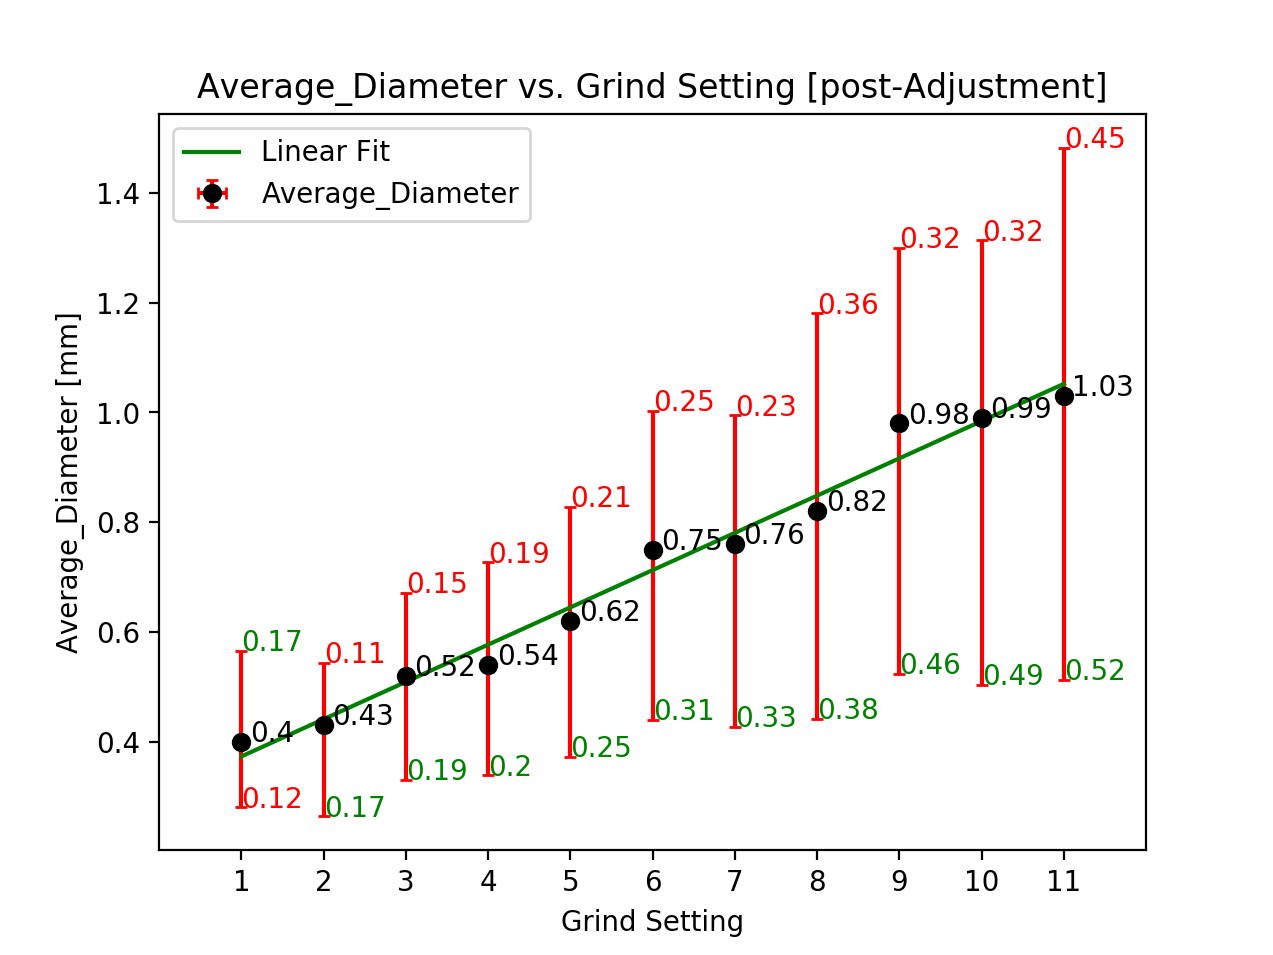
\includegraphics[width=\columnwidth]{postAdjustmentAverage_DiameterPlot.png}\caption{Post-Adjustment Plot}\label{fig:postAdjustmentGraph}\end{figure}\end{center}

\section{Results Analysis}

An additional factor indicating the grinder needed adjustment was an audible skipping sound if the burrs were made to touch just below grind setting one. The burrs should not touch to begin with, and if they do should produce a continuous rubbing sound. Instead the sound indicated the burr faces were not perfectly parallel. \\

After adjusting and aligning the burrs a test sample was run through the grinder and two observations were made. Firstly, once the primary mass of coffee was ground, the duration residual particles remained in the grinding chamber was noticeably reduced. No time was measured prior to adjustment so we are unable to quantify this change exactly. Second, when adjusting to just below grind setting one[4], the burrs made a subtle continuous rubbing sound instead of the skipping sound heard pre-adjustment. \\

The greatest improvements pre-adjustment and post-adjustment are noticeable in the highest and lowest grind settings shown in Figures \ref{fig:preAdjustmentGraph} and \ref{fig:postAdjustmentGraph}. Grind settings one through four pre-adjustment show little to no grind-adjustment resolution with one through three having nearly the same value and four only slightly coarser. Grind settings two and three have the same average value yet different left and right standard deviations, perhaps indicative of the variable extraction we tasted. At the high end grind settings ten and eleven pre-adjustment have much higher average changes from their previous settings, $\Delta=0.12$ and $0.14$ respectively, as well as a much larger boulders production in setting eleven compared to post-adjustment.\\

Linearity also increased post-adjustment as seen by the tighter grouping in Figure \ref{fig:postAdjustmentGraph} as well as the higher $R^2$ value shown in Table 1. Left and right standard deviations decreased in some grind settings but increased in others, however overall there is still more spread in grind size than anticipated. \\

\section{Conclusion}

The condition of a 2015 Mahlkonig EK-43 was tested using an open source program coffeegrindsize(1) enabling quantitative measurement of particles often too small to measure accurately or efficiently. Using data from this program it was shown with supplementary Python code(5) the grinder was in need of adjustment and alignment, confirmed by lack of adjustment resolution in lower grind settings and non-linearity of average grind sizes through the grinding range. The grinder's sub-optimal performance was also noted anecdotally during regular tastings and has, to a great extent, improved since these procedures were carried out. Coffeegrindsize also quantified grind size distribution for a particular setting further indicating the burr's condition.

This first project provided guidance how grind samples should be taken in future projects with greater precision in mind. Hopefully new burrs provide a tighter distribution in grind size to make grinder-to-grinder correlation meaningful. 

If you have any comments, questions, or reflections please email me at \url{frothGoth@protonmail.com}

\section{References}
(1) J Gagne's Blog about coffeegrindsize\\
\url{https://coffeeadastra.com/2019/04/07/an-app-to-measure-your-coffee-grind-size-distribution-2/}\\\\
(2) Coffeegrindsize source Code\\
\url{https://github.com/jgagneastro/coffeegrindsize/blob/master/coffeegrindsize.py}\\\\
(3) Manual for coffeegrindsize\\
\url{https://github.com/jgagneastro/coffeegrindsize/blob/master/Help/coffee_grind_size_manual.pdf}\\\\
(4) Barista Hustle Alignment Video\\
\url{https://www.youtube.com/watch?v=5-cf0Iack5Q}\\\\
(5) My github for supplementary code\\
\url{https://github.com/TopDownTom/coffeeMisc}\\\\
(6) Scipy curve\_\ fit documentation\\
\url{https://docs.scipy.org/doc/scipy/reference/generated/scipy.optimize.curve_fit.html}\\\\


\end{document}